\documentclass[11pt]{beamer}
\usetheme{Antibes}
\usepackage[utf8]{inputenc}
\usepackage{amsmath}
\usepackage{amsfonts}
\usepackage{amssymb}
%\usepackage{biblatex}
\usepackage[backend=bibtex]{biblatex} 
\graphicspath{{images/}}
%\author{}
%\title{}
%\setbeamercovered{transparent} 
%\setbeamertemplate{navigation symbols}{} 
%\logo{} 
%\institute{} 
%\date{} 
\subject{GPU Architecture} 
\addbibresource{HMM.bib}
\begin{document}

\begin{frame}
\title{HMM Inference with CUDA}
\subtitle{Marc Haubenstock \& Christian Brändle}

\titlepage
\end{frame}

%\begin{frame}
%\tableofcontents
%\end{frame}

\begin{frame}{Introduction}

A \emph{Hidden Markov Model} describe a \textbf{two-state stochastic process}.
There is a stochastic process that is stationary (which means its probabilistic features don't change over time) and a state space that is finite.

\end{frame}

\begin{frame}{Introduction cont.}
% figure for state transition table as finite state automaton
\begin{table}[h]
	\begin{center}
		\begin{tabular}{| c | c |}
			\hline
			\multicolumn{2}{|l|}{
				\begin{tabular}{ l }
					\emph{Finite state automatons} \\
				\end{tabular}
			} \\
			\hline
			& \\
			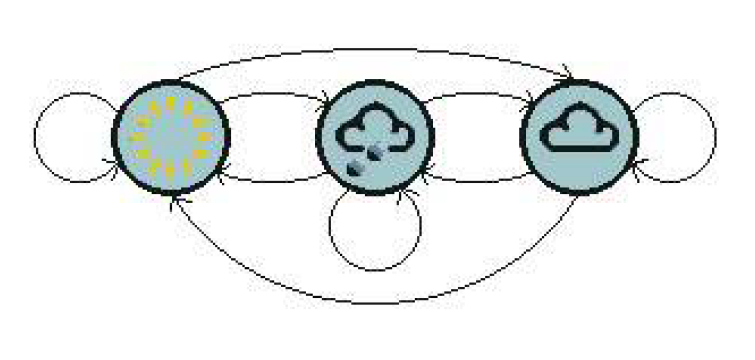
\includegraphics[width=0.25\textwidth]{./Images/FiniteStateAutomaton_1.png} & 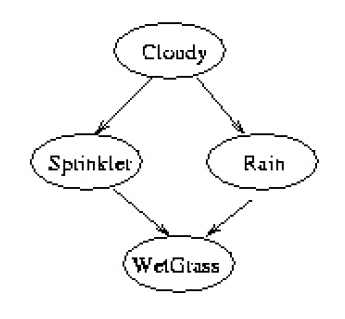
\includegraphics[width=0.25\textwidth]{./Images/FiniteStateAutomaton_2.png} \\
			\hline
			weather HMM \footcite{hmm_fb} & grass HMM \footcite{gm_bn} \\
			\hline
		\end{tabular}
	\end{center}
	\caption{Two finite state automatons that describe the state space of two different HMMs. Nodes correspond to states and edges to transition probabilites betwenn states that are bigger than $0$.}
	\label{tab:FiniteSA}
\end{table}


\end{frame}

\begin{frame}{Introduction cont.}
The important thing is that \textbf{the behaviour of the process given at time $t$ only depends on the immediate predecessor state}.

So the \emph{Markov property} states:

\begin{equation}
	P(S_t | S_1,S_2, \ldots S_{t-1}) = P(S_t | S_{t-1})
\end{equation}
\end{frame}

\begin{frame}{Introduction cont.}
Visually this can be shown with a graph model of a HMM as a sequence of hidden states $X_i$ and the corresponding obervations $Y_i$ - see figure \ref{fig:GraphModel}.

% GraphModelHMM_1.png
\begin{figure}[H]
	\centering
	
	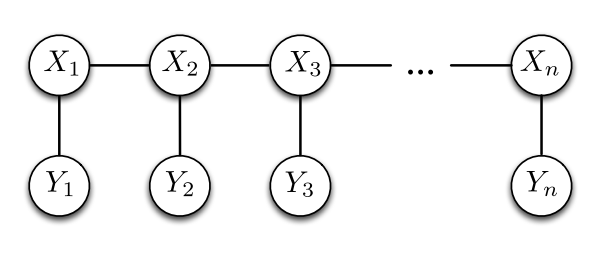
\includegraphics[width=0.66\textwidth]{./Images/GraphModelHMM_1.png}
	\caption{ \cite{hmm_II}}
	\label{fig:GraphModel}
\end{figure}

\end{frame}

\begin{frame}{Introduction cont.}
Furthermore, the corresponding \textbf{probability distribution only depend on the current state}. This is called the \emph{output independence assumption}.

\begin{equation}
P(O_t | O_1,O_2, \ldots O_{t-1}) = P(O_t | S_{t-1})
\end{equation}

The model itself is 'hidden' because we only can observe the outputs generated, namely the \emph{observation sequence} $O_1, O_2, \ldots,  O_T$.
\end{frame}

\begin{frame}{Introduction cont.}
\begin{figure}
\includegraphics[scale=0.25]{"symbols"}
\end{figure}
\end{frame}

\begin{frame}{Algorithms}
\begin{figure}[H]

\centering
\includegraphics[scale=0.4]{"FW"}
 \caption{Pesudo-Code for the Forward Algorithm \cite{cuhmm}}

\end{figure}

\end{frame}

\begin{frame}{Algorithms}
\begin{figure}[H]

\centering
\includegraphics[scale=0.4]{"vit"}
 \caption{Pesudo-Code for the Viterbi Algorithm \cite{cuhmm}}

\end{figure}
\end{frame}

\begin{frame}{Algorithms}
\begin{figure}[H]

\centering
\includegraphics[scale=0.3]{"BW"}
 \caption{Pesudo-Code for the Backward Forward Algorithm \cite{cuhmm}}

\end{figure}
\end{frame}

\begin{frame}{Algorithms}
\begin{figure}[H]

\centering
\includegraphics[scale=0.4]{"estimation"}
 \caption{Estimation of the A and B Matricies \cite{cuhmm}}

\end{figure}

The estimated values of the emission matrix B is not dependent on \(\epsilon(j)\), but should be on \(\gamma\), as it is defined in literature \cite{hmm}. 
\end{frame}

\begin{frame}{Implementation}
\begin{figure}[H]
\centering

\includegraphics[scale=0.2]{"3d_trellis"}
  \caption{Graphical representation of the data structure presented in \textit{A Cuda Implementation of Hidden Markov Models}\cite{cuhmm}}
\end{figure}
\end{frame}

\begin{frame}{Implementation cont.}
\begin{center}

\( D_{ij} = B_{O_i} .* C_i \times A_j \)

\end{center}

Where \( B_{O_i}\) is the row of the emission matrix at observation \(O_i\), \(C_i\) is the previous slice and \(A_j\) is the j\textsuperscript{th} column of the transition. matrix A.
\end{frame}

\begin{frame}{Implementation cont.}
\begin{figure}[H]
\centering

\includegraphics[scale=0.2]{"slice"}
  \caption{The computation of a slice\cite{cuhmm}}
\end{figure}
\end{frame}

\begin{frame}{Implementation cont.}
Finally a stipulation of the outlined method is that:

\begin{itemize}
\item The number of states and sequences must be a multiple of block size 16
\item The number of output sequences must be of the same length.
\end{itemize}
\end{frame}

\begin{frame}[fragile]{Forward}
\begin{verbatim}
	__global__ initTrellis<<<M,N>>>(..){
	int obs_index = blockIdx.x * T_noOfObservations;
	int obs_start = dev_O_obsSequences_2D[obs_index];
	int idx_b_i_idxOs = threadIdx.x*V_noOfObsSymbols 
	+ obs_start;
	int idx_alpha_0i = blockIdx.x * N_noOfStates 
	+ threadIdx.x;
	int idx_pi_i = threadIdx.x;

	double alpha_0_i 
	= dev_Pi_startProbs_1D[idx_pi_i] * dev_B[idx_b_i_idxOs];
	dev_3D_Trellis[idx_alpha_0i] = alpha_0_i;
	}

\end{verbatim}
\end{frame}

\begin{frame}[fragile]{Forward}
\begin{verbatim}
// Computes the B matrix in term D = B .* C x A
	ComputeBDevice << < M, N >> >
	(M, V, T, N, 
	dev_O_obsSequence_2D, dev_B_obsEmissionProbs_2D, i, dev_B);

	// All dimensions are multipe of Warp Sizes
	// Compute W =  B .* C
	pointwiseMatrixMul << <M, N >> >(dev_W, dev_B,
	&dev_3D_Trellis[(i - 1) * M * N]);

	// Compute D = W x A
	cublasMultiplyDouble(M, N_noOfStates, N, dev_W, 
	dev_A_stateTransProbs_2D, &dev_3D_Trellis[i * M * N]);
\end{verbatim}
\end{frame}

\begin{frame}[fragile]{Forward}
\begin{verbatim}
__global__ void ComputeBDevice(...){
	
	// index to access element of B matrix
	unsigned int idx = blockIdx.x * blockDim.x + threadIdx.x;
	// index to access device_Obs_seq
	int idx_m_ij = blockIdx.x *T_noOfObservations + j;
	unsigned int value = dev_O_obsSequences_2D[idx_m_ij];

	int emission_idx = value * V_noOfObsSymbols + threadIdx.x;
	dev_B[idx] = dev_B_obsEmissionProbs_2D[emission_idx];

}
\end{verbatim}
\end{frame}

\begin{frame}[fragile]{Forward}
\begin{verbatim}
__global__ void ComputeBDevice(...){
	
	// index to access element of B matrix
	unsigned int idx = blockIdx.x * blockDim.x + threadIdx.x;
	// index to access device_Obs_seq
	int idx_m_ij = blockIdx.x *T_noOfObservations + j;
	unsigned int value = dev_O_obsSequences_2D[idx_m_ij];

	int emission_idx = value * V_noOfObsSymbols + threadIdx.x;
	dev_B[idx] = dev_B_obsEmissionProbs_2D[emission_idx];

}
\end{verbatim}
\end{frame}

\begin{frame}[fragile]{Forward}
\begin{verbatim}
	for (int i = 0; i < M_noOfObsSequences; i++)
	{

		int smBytes = 64 * sizeof(double);
		int grid = N_noOfStates / 64;
		reduce_1 <<< grid, 64, smBytes >>>
		(&last_slice[i*N_noOfStates], dev_A_odata);

		memcpyVector(..);

		host_likelihoods_1D[i] = host_A_odata[0] + host_A_odata[1];

	}
\end{verbatim}
\end{frame}


\begin{frame}[fragile]{Forward}
\begin{verbatim}
	for (int i = 0; i < M_noOfObsSequences; i++)
	{

		int smBytes = 64 * sizeof(double);
		int grid = N_noOfStates / 64;
		reduce_1 <<< grid, 64, smBytes >>>
		(&last_slice[i*N_noOfStates], dev_A_odata);

		memcpyVector(..);

		host_likelihoods_1D[i] = host_A_odata[0] + host_A_odata[1];

	}
\end{verbatim}
\end{frame}

\begin{frame}[fragile]{Viterbi}
	\begin{verbatim}
	
	\end{verbatim}
\end{frame}

\end{document}